%!TEX root = mieic.tex
\chapter{Solução Implementada} \label{chap:sol}

\section*{}

Neste capítulo é descrita de forma pormenorizada a solução implementada de modo a responder aos desafios colocados na introdução, cumprindo assim os objetivos propostos.
Inicialmente é caracterizada a arquitetura definida, fazendo referência aos diferentes modulos que constituem o “produto” final. Posteriormente são referidas de uma forma breve as tecnologias envolvidas no seu desenvolvimento.


\section{Visão Geral} \label{sec:geral}

Tal como foi referido na definição dos objetivos, era esperado o desenvolvimento e validação de uma arquitectura que permitisse uma interação baseada na manipulação direta, através de um dispositivo móvel, facilitando a criação de aplicações para ecrãs públicos.  
Na solução encontrada, de uma maneira global, é possível diferenciar três diferentes componentes, sendo eles o servidor, desenvolvido em node.js, a aplicação, que irá correr no servidor criado comunicando com este através de \textit{web sockets} e ainda o utilizador final, aqui identificado como cliente.
A FIGURA apresenta, de uma forma simples, os componentes acima descritos.
\missingfigure{Diagrama de componentes}

A [inserir num fig] representa um diagrama de sequência mostrando as diferentes interações entre os componentes constituintes do sistema implementado. Inicialmente terá de existir um pedido por parte de um ecrã para aceder à aplicação, neste momento a aplicação comunica com o servidor e a partir daqui está preparada para pedidos de possíveis utilizadores. Um utilizador, ao querer interagir com a aplicação está a enviar um pedido para esta, que por sua vez avisa o servidor e este é responsável por mostrar no dispositivo o widget da aplicação. Neste momento o widget liga-se ao servidor e após ocorrer a ligação procede-se à troca de “mensagens” que permitem ao utilizador definir o seu nome, quando o cliente tiver o nome definido pode usufruir do widgets disponíveis, realizando-se a comunicação do  widget para o servidor, que por sua vez envia para a aplicação.
\missingfigure{Diagrama de sequência}


\section{Tecnologias Usadas} \label{sec:tec}

Ao longo da implementação houve necessidade de optar por diversas tecnologias para que fosse possível alcançar o objetivo desejado, Node.js foi usado para a implementação do servidor e \textit{web sockets} e \textit{socket.io} para facilitar a comunicação entre os diversos componentes. Foi também usada a \textit{framework} \textit{Prototype} que pemrite a manipulação de classes em \textit{JavaScript}, e uma biblioteca, \textit{Swipeable} que dá resposta a eventos swipe facilitando a utilização.

\begin{itemize}

\item \textbf{Node.js}


\textit{Node.js} é uma plataforma construída para facilitar o desenvolvimento de aplicações de alta escalabilidade em tempo real, com base no interpretador \textit{Javascript V8} da \textit{Google}, que antes da execução compila \textit{JavaScript} em código máquina, melhorando consideravelmente o tempo de execução. Deste modo Node permite a construção de aplicações rápidas e altamente concorrentes.

Segundo Michael Abernethy ~\cite{Abernethy2011} node altera a noção de como um servidor deve funcionar, referindo que o seu objetivo é permitir que um programador construa applicações com grande escalabilidade e que o código desenvolvido suporte milhares de ligaçõe simultâneasa numa só máquina. 

\textit{Node.js} opera uma \textit{thread} simples, usando chamadas E/S “que não bloqueiam”(non-blocking), permitindo o suporte das diversas ligações ~\ref{fig:node}.

\begin{figure}[ht]
\centering
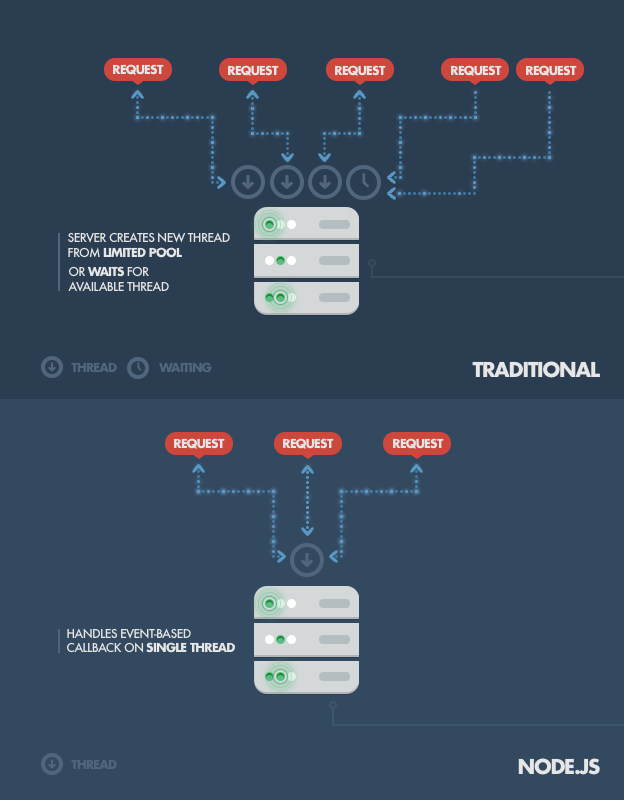
\includegraphics[width=0.5\columnwidth]{node.png}
\caption[\textit{Node.js}] {Diferença entre técnicas tradicionais de servidores e \textit{Node.js}\protect\footnotemark}
\label{fig:node}
\end{figure}

\footnotetext{http://www.toptal.com/nodejs/why-the-hell-would-i-use-node-js}

\item \textbf{Web Sockets}

De forma a permitir a comunicação do utilizador, lado do cliente, com o servidor criado foram usados web sockets. Estes foram desenvolvidos para serem implementados em em aplicações ou servidores web, usando um protocolo independente baseado em TCP.

O protocolo websocket encontra-se standardizado, o que significa que é seguida uma norma no envio de informação entre o servidor e o “browser” sem que haja uma solicitação por parte do cliente o que possibilita uma maior interação entre estes, facilitando a criação de aplicações em tempo real. É deste modo criada uma ligação bi-direcional entre o \textit{browser} e o servidor, pois a conexão é mantida aberta enquanto as mensagens são encaminhadas de um lado para o outro.


\item \textbf{Socket.io}

Socket.io é descrita como uma biblioteca javascript usada no desenvolvimento de aplicações web. Esta é composta por 2 partes, uma biblioteca para o lado do cliente, que corre no browser, e outra para o lado do servidor, que para terá de ser implementado em node.js, daí este estar acima referido como uma das tecnologias usadas. Quer o lado do cliente quer o do servidor apresentam “API’s” idênticas. 
Usa, principalmente como protocolo, websockets, também escolhido como tecnologia usada no desenvolvimento desta solução, contudo, se necessário, podem ser utilizados outros, como por exemplo Adobe Flash sockets, JSONP polling, and AJAX long polling. 
A sua escolha aliada a websockets fornece bastante recursos, como a transmissão para múltiplos sockets, armazenamento de informação associada a cada cliente e ainda “inputs/outputs” assíncronos. 

\item \textbf{Prototype}

Prototype é uma \textit{framework} em \textit{JavaScript} que fornece algumas funções para o desenvolvimento de aplicações em \textit{JavaScript}. As suas funcionalidades variam entre pequenos atalhos de programação e principais funções para lidar com \textit{XMLHttpRequest}.

Esta \textit{framework} fornece ainda uma biblioteca com funções que suporta classes e objetos baseados em classes, algo que não é possível em \textit{JavaScript}.

\item \textbf{Swipeable}

Swipeable trata-se de uma biblioteca que permite obter resposta a eventos \textit{swipe} realizados num dispositivo \textit{touch}, sendo uma abstração do \textit{touchstart}, \textit{touchmove} e \textit{touchend}. 
Foi incluída no ficheiro widget.js de para possibilitar o desenvolvimento e correto funcionamento do widget “SWIPE”.

\end{itemize}


\section{Framework Desenvolvida} \label{sec:framework}

\subsection{API}

\subsection{Controlos Definidos}

	A API desenvolvida apresenta três diferentes tipos de controlos que o programador terá à sua disposição para implementar, de acordo com aplicação desenvolvida. Neste momento existem como possíveis opções, o \textit{joystick}, o \textit{swipe} e ainda outro composto por uma caixa de introdução de texto.

	\begin{itemize}

	\item \textbf{Joystick}

		Controlo composto pelas quatro setas tradicionais, esquerda, direita, cima e baixo, que pode ser utilizado em qualquer aplicação que exija uma movimentação.

	\item \textbf{Swipe}

		Controlo que usa as propriedade touch do dispositivo para controlar a aplicação, definido apenas para reconhcer uma direção, contudo pode ser alterado.

	\item \textbf{InputText}

		Controlo que permite ao utilizador a interação com aplicações que exijam a introdução de texto.

	\end{itemize}


	
\subsection{Aplicações Exemplo}

	Neste momento apenas existe uma aplicação exemplo, no entanto permite ao utilizador o uso dos três tipos de controlo disponíveis.
	



